
\documentclass[twocolumn,10pt]{article}
\title{Constructing triangles}
\setlength{\columnsep}{20pt} 
\usepackage{amsmath,hyperref,cancel,graphicx}
 \def\shrinkfactor{0.45}
 \usepackage[margin=1.5cm]{geometry}
\usepackage[usenames,dvipsnames]{color}
 
 \newcommand{\blue}[1]{{\color{Blue}#1}} 
 \newcommand{\purple}[1]{{\color{Purple}#1}} 
 \newcommand{\red}[1]{{\color{Red}#1}} 
 \newcommand{\green}[1]{{\color{Green}#1}} 
 \newcommand{\gray}[1]{{\color{Gray}#1}} 
  \newcommand{\pink}[1]{{\color{Magenta}#1}}   


\begin{document}
\maketitle



\section{\href{https://www.khanacademy.org/devadmin/content/items/x0a2c8d4a7e3a85b9}{x0a2c8d4a7e3a85b9}}

\noindent
**How many triangles can be drawn where the side length is known between two known angles?**

\paragraph{Ans} 

None

\fbox{ Only one

}

 More than one



\paragraph{Hint 1}A triangle is a plane figure with $3$ straight sides and $3$ angles. Can we satisfy the definition given the conditions? Let's try to draw a triangle where the side length is known between $2$ angles.

\paragraph{Hint 2}The $3$ angles in a triangle always sum to $180^\circ$. Because we know the measure of $2$ angles, we can find the measure of the third angle.

\paragraph{Hint 3}Let's draw any triangle where we know the side length between $2$ known angles. For example, let's look at when a side of length $5$ is between $2$ equal angles $75^\circ$ and $75^\circ$. The other $2$ sides must be equal and meet at a $30^\circ$ angle. 


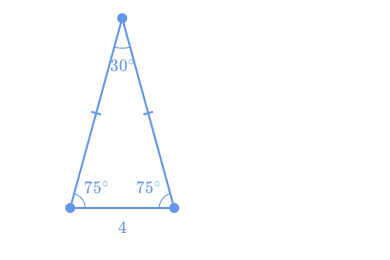
\includegraphics[scale=\shrinkfactor]{figures/8664b06c420b8bf33711310103a6963e0f2cc7f1.png}

This triangle is unique, meaning no other triangle exists with exact same shape or size.

\paragraph{Hint 4}If  the side length is known between two known angles, only one triangle can be drawn.



\medskip
\noindent
\textbf{Tags:} {\footnotesize Constructing triangles, CC.7.G.A.2}\\
\textbf{Version:} d920ceb5.. 2013-10-18
\smallskip\hrule





\section{\href{https://www.khanacademy.org/devadmin/content/items/x18341f6f8d24d96e}{x18341f6f8d24d96e}}

\noindent
**How many triangles can be drawn with side lengths $9$, $12$ and $15$?**

\paragraph{Ans} 

None

\fbox{ Only one

}

 More than one



\paragraph{Hint 1}A triangle is a plane figure with $3$ straight sides and $3$ angles. Can we satisfy the definition given the conditions? Let's try to draw a triangle given the conditions.

\paragraph{Hint 2}In general, the longest side of a triangle must be shorter than the sum of the two other sides. Because $\blue{9}+\blue{12} =\blue{21}$, the two sides $\blue{9}$ and $\blue{12}$ meet to form $2$ angles with the side of length $\blue{15}$. We can create $3$ angles with the $3$ sides to satisfy the definition of a triangle.


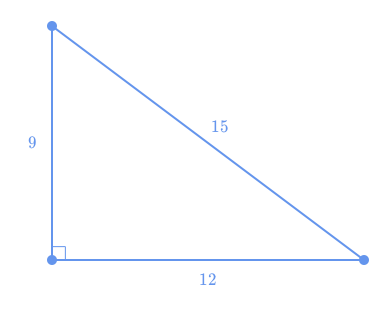
\includegraphics[scale=\shrinkfactor]{figures/9e3335e4646b2e59f3ceb8860cd9099de97f22b0.png}

\paragraph{Hint 3}Given the conditions, only one triangle can be drawn.



\medskip
\noindent
\textbf{Tags:} {\footnotesize Constructing triangles, CC.7.G.A.2}\\
\textbf{Version:} 4c858421.. 2013-10-18
\smallskip\hrule





\section{\href{https://www.khanacademy.org/devadmin/content/items/x1afa3df30210708e}{x1afa3df30210708e}}

\noindent
**Draw a triangle with side lengths $5a$,  $12a$ and $13a$ where $a>0$.**

**Given these criteria is the triangle unique?**
[[? interactive-graph 1]]

\paragraph{Ans} 

Yes

\fbox{ No

}

 

\paragraph{Hint 1}Let�s start by choosing a value for $\pink{a}$ where $\pink{a}>0$, then we can draw a triangle with side lengths $\purple5\pink{a}$, $\purple{12}\pink{a}$ and $\purple{13}\pink{a}$.

\paragraph{Hint 2}If $\pink{a}=1$, then we can draw a triangle with side lengths  $\blue{5}$, $\blue{12}$ and $\blue{13}$. This is a right triangle. 


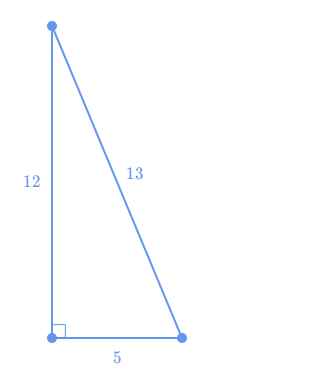
\includegraphics[scale=\shrinkfactor]{figures/6d298ed14c507f692b6d88792d963d7008b9847a.png}

\paragraph{Hint 3}If $\pink{a}=0.5$, then we can draw a right triangle with side lengths $\blue{2.5}$, $\blue{6}$ and $\blue{6.5}$.

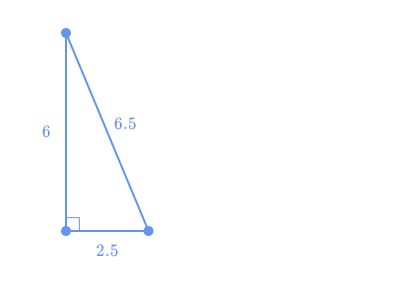
\includegraphics[scale=\shrinkfactor]{figures/463955e595c31361c49d853aea12289b0f5f7779.png}

We can let $\pink{a}$ be any nonzero positive number and draw many triangles of same shape but different sizes.

\paragraph{Hint 4}The triangle is not unique. 


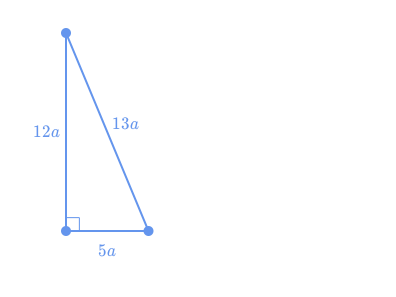
\includegraphics[scale=\shrinkfactor]{figures/28bab6f73b266fa0cb6392a48f06caca532f0cd2.png}



\medskip
\noindent
\textbf{Tags:} {\footnotesize Constructing triangles, CC.7.G.A.2}\\
\textbf{Version:} 5e8d2d2a.. 2013-10-18
\smallskip\hrule





\section{\href{https://www.khanacademy.org/devadmin/content/items/x1c875467bbf94500}{x1c875467bbf94500}}

\noindent
**Draw a triangle with side length $4$ between two $70^\circ$ angles.** 

**Given these criteria is the triangle unique?**
[[? interactive-graph 1]]

\paragraph{Ans} 

\fbox{ Yes

}

 No



\paragraph{Hint 1}Let�s start by drawing the length of $1$ side, which we know is $\blue4$.  

\paragraph{Hint 2}From the side $\blue4$, let�s draw $2$ $\blue{70^\circ}$ angles. Since we have $2$ equal angles, we have an isosceles triangle. An isosceles triangle has at least $2$ sides equal in length. 

Since we have $2$ $\blue{70^\circ}$ angles, the third angle must be $\green{40^\circ}$. The sum of $3$ angles in a triangle will always be $\pink{180^\circ}$.

\paragraph{Hint 3}We know the measure of $2$ angles and the length of the side between the angles, so we can draw only $1$ triangle.

\paragraph{Hint 4}The triangle is unique.


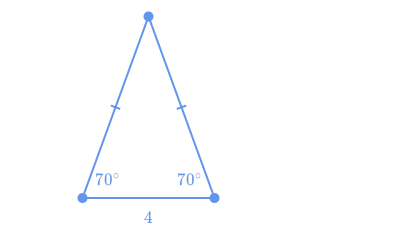
\includegraphics[scale=\shrinkfactor]{figures/42e1efd00be59b64d19c796b09c66213066bd2fa.png}



\medskip
\noindent
\textbf{Tags:} {\footnotesize Constructing triangles, CC.7.G.A.2}\\
\textbf{Version:} 7ec6851f.. 2013-10-17
\smallskip\hrule





\section{\href{https://www.khanacademy.org/devadmin/content/items/x1da87b180aca0e3d}{x1da87b180aca0e3d}}

\noindent
**How many triangles can be drawn side lengths of $5$ and $10$?**

\paragraph{Ans} 

None

Only one

\fbox{ More than one

}

 

\paragraph{Hint 1}Without knowing at least $1$ angle measure, we cannot create a unique triangle with only one shape and size.

\paragraph{Hint 2}We can  draw many triangles with side lengths $\blue5$ and $\blue{10}$.


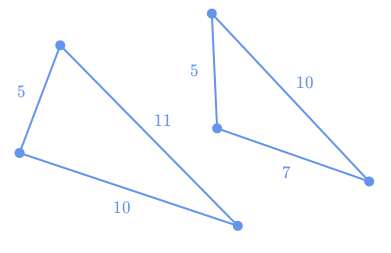
\includegraphics[scale=\shrinkfactor]{figures/fe9bb66c73daee381242a48159a578e8b78ac0fb.png}

\paragraph{Hint 3}If we only know $1$ angle and $1$ side length, more than one triangle can be drawn.



\medskip
\noindent
\textbf{Tags:} {\footnotesize Constructing triangles, CC.7.G.A.2}\\
\textbf{Version:} 37208764.. 2013-10-18
\smallskip\hrule





\section{\href{https://www.khanacademy.org/devadmin/content/items/x25470998d7b41ee4}{x25470998d7b41ee4}}

\noindent
**How many triangles can be drawn where side length $2$ is not between two $45^\circ$ angles?**

\paragraph{Ans} 

None

\fbox{ Only one

}

 More than one



\paragraph{Hint 1}A triangle is a plane figure with $3$ straight sides and $3$ angles. The $3$ angles always add up to $\pink{180^\circ}$. 

We have $2$ $\blue{45^\circ}$ angles.  Since $\pink{180^\circ}-2\cdot\blue{45^\circ}=\blue{90^\circ}$, the missing angle is $\blue{90^\circ}$. We have a right triangle. 

\paragraph{Hint 2}We know a length and $2$ angles. We can draw a triangle given the side length $\blue2$ is not between the $2$ $\blue{45^\circ}$ angles. The side length $\blue2$ is between the $\blue{45^\circ}$ and $\blue{90^\circ}$ angles:


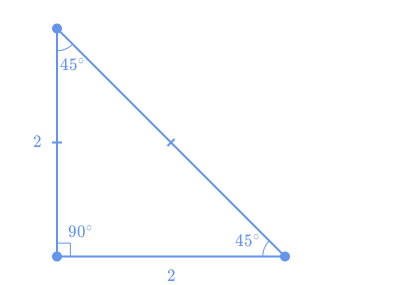
\includegraphics[scale=\shrinkfactor]{figures/50ab52075216ec1ebe030aa80de8615558c71846.png}

This triangle is unique, meaning no other triangle exists with exact same shape or size.

\paragraph{Hint 3}Given the conditions, only one triangle can be drawn.



\medskip
\noindent
\textbf{Tags:} {\footnotesize Constructing triangles, CC.7.G.A.2}\\
\textbf{Version:} 4890bf29.. 2013-10-18
\smallskip\hrule





\section{\href{https://www.khanacademy.org/devadmin/content/items/x2bce84b97313fd2b}{x2bce84b97313fd2b}}

\noindent
**Draw a triangle where the side length $3$ is not between two angles $31^\circ$ and $90^\circ$.**

**Given these criteria is the triangle unique?**
[[? interactive-graph 1]]

\paragraph{Ans} 

\fbox{ Yes

}

 No



\paragraph{Hint 1}Let�s start by drawing a right angle which is $\blue{90^\circ}$. 

Then, let's draw the side of length $\blue3$ next to the right angle, so our base is length $\blue3$.

\paragraph{Hint 2}The length of $\blue3$ is $\red{\text{not}}$ between $2$ angles $\blue{31^\circ}$ and $\blue{90^\circ}$. 

Since we drew the side of length $\blue3$ next to the right angle, the $\blue{31^\circ}$ angle must be *opposite* the side of length $\blue3$ .

\paragraph{Hint 3}We know the measure of $2$ angles and the length of $1$ side not between the angles, so we can draw only $1$ triangle.

\paragraph{Hint 4}The triangle is unique.


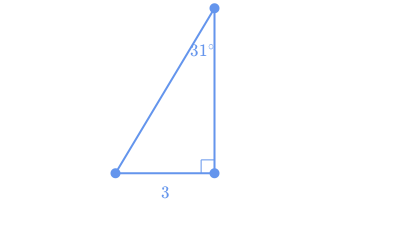
\includegraphics[scale=\shrinkfactor]{figures/48773248b446b970cdf6c2fa7664c3fa8890378a.png}



\medskip
\noindent
\textbf{Tags:} {\footnotesize Constructing triangles, CC.7.G.A.2}\\
\textbf{Version:} 1215aaf1.. 2013-10-17
\smallskip\hrule





\section{\href{https://www.khanacademy.org/devadmin/content/items/x31c216ff88dad8e7}{x31c216ff88dad8e7}}

\noindent
**How many triangles can be drawn with side lengths $4$, $4$ and $7$?**

\paragraph{Ans} 

None

\fbox{ Only one

}

 More than one



\paragraph{Hint 1}A triangle is a plane figure with $3$ straight sides and $3$ angles. Can we satisfy the definition given the conditions? Let's try to draw a triangle given the conditions.

\paragraph{Hint 2}In general, the longest side of a triangle must be shorter than the sum of the two other sides. Because $\blue{4}+\blue{4} =\blue{8}$, the two sides $\blue{4}$ and $\blue{4}$ meet to form $2$ angles with the side of length $\blue{7}$. We can create $3$ angles with the $3$ sides to satisfy the definition of a triangle.


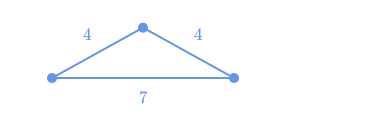
\includegraphics[scale=\shrinkfactor]{figures/a5961a517a4e6e5e6def530e3948dc049dbfad9a.png}

\paragraph{Hint 3}Given the conditions, only one triangle can be drawn.



\medskip
\noindent
\textbf{Tags:} {\footnotesize Constructing triangles, CC.7.G.A.2}\\
\textbf{Version:} 13a63a31.. 2013-10-18
\smallskip\hrule





\section{\href{https://www.khanacademy.org/devadmin/content/items/x38cc51ab93842600}{x38cc51ab93842600}}

\noindent
**How many triangles can be drawn with side lengths $1$, $1$ and $2$?**

\paragraph{Ans} 

\fbox{ None

}

 Only one

More than one



\paragraph{Hint 1}A triangle is a plane figure with $3$ straight sides and $3$ angles. Can we satisfy the definition given the conditions? Let's try to draw a triangle given the conditions.

\paragraph{Hint 2}In general, the longest side of a triangle must be shorter than the sum of the two other sides. Because $\blue{1}+\blue{1} =\blue{2}$, the two side lengths $\blue{1}$ and $\blue{1}$ cannot meet to form a third angle. We cannot create $3$ angles to satisfy the definition of a triangle.

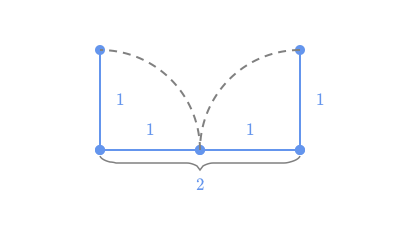
\includegraphics[scale=\shrinkfactor]{figures/0fc8a765d9e1e79a7c3e4874b8f9448d3b5c1d18.png}

\paragraph{Hint 3}Given the conditions, no triangles can be drawn.



\medskip
\noindent
\textbf{Tags:} {\footnotesize Constructing triangles, CC.7.G.A.2}\\
\textbf{Version:} aeb719e4.. 2013-10-18
\smallskip\hrule





\section{\href{https://www.khanacademy.org/devadmin/content/items/x4c335bfbee0cba92}{x4c335bfbee0cba92}}

\noindent
**Draw a right triangle with at least $2$ side lengths equal.** 

**Given these criteria is the triangle unique?**
[[? interactive-graph 1]]

\paragraph{Ans} 

Yes

\fbox{ No

}

 

\paragraph{Hint 1}Let�s start by drawing. A right triangle has one $\blue{90 ^\circ}$angle. 

A triangle with at least $2$ side lengths equal is isosceles. We do not know the side lengths.

\paragraph{Hint 2}Since we are given the measures of $3$ angles and do not know any side lengths, we can draw many triangles with at least $2$ side lengths equal.

\paragraph{Hint 3}The triangle is not unique.

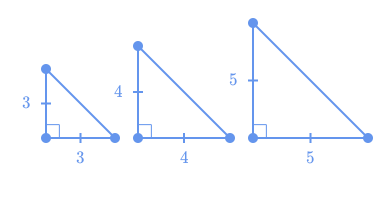
\includegraphics[scale=\shrinkfactor]{figures/d8b2dd5b2d43266692ba3d2c35cf5638f2f3c05c.png}



\medskip
\noindent
\textbf{Tags:} {\footnotesize Constructing triangles, CC.7.G.A.2}\\
\textbf{Version:} 0abcb8e1.. 2013-10-18
\smallskip\hrule





\section{\href{https://www.khanacademy.org/devadmin/content/items/x531e157ba7c498eb}{x531e157ba7c498eb}}

\noindent
**How many triangles can be drawn where the measures of all $3$ angles are known?**

\paragraph{Ans} 

None

Only one

\fbox{ More than one

}

 

\paragraph{Hint 1}A triangle is a plane figure with $3$ straight sides and $3$ angles. Can we satisfy the definition given the conditions? Let's try to draw a triangle where we known the lengths of all $3$ angles.

\paragraph{Hint 2}For example, let's look at when all $3$ angles are $\blue{60^\circ}$:


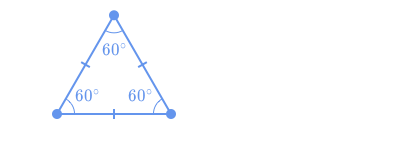
\includegraphics[scale=\shrinkfactor]{figures/9bbd0fa30a5ae16d50c816c4a8c4cfc44a68146c.png}

Is this triangle unique, meaning do no other triangles exist with exact same shape or size?

\paragraph{Hint 3}We can draw many equilateral triangles with same shape but different sizes:


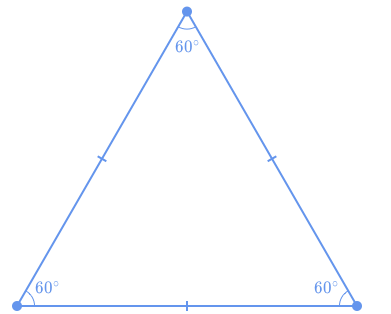
\includegraphics[scale=\shrinkfactor]{figures/3e0462daa95058cdd7264a43f9c163723c418fd6.png}

\paragraph{Hint 4}If the measures of all $3$ angles are known, more than one triangle can be drawn.



\medskip
\noindent
\textbf{Tags:} {\footnotesize Constructing triangles, CC.7.G.A.2}\\
\textbf{Version:} a46c4b72.. 2013-10-18
\smallskip\hrule





\section{\href{https://www.khanacademy.org/devadmin/content/items/x572fecbc70b353aa}{x572fecbc70b353aa}}

\noindent
**Draw an isosceles right triangle with two side lengths $3$.** 

**Given these criteria is the triangle unique?**
[[? interactive-graph 1]]

\paragraph{Ans} 

\fbox{ Yes

}

 No



\paragraph{Hint 1}Let�s start by drawing. A right triangle has one $\blue{90 ^\circ}$angle. 

An isosceles triangle has at least $2$ side lengths equal. We are given $2$ side lengths both equal to $\blue3$. 

\paragraph{Hint 2}Let's draw $1$ side length $\blue{3}$ as the height vertically (up and down) from the $\blue{90 ^\circ}$angle. Let's draw the other side length $\blue{3}$ as the base horizontally (left and right) from the $\blue{90 ^\circ}$angle. 

\paragraph{Hint 3}Since we are given the measures of $2$ sides and the angle between them, we can draw only $1$ triangle.

\paragraph{Hint 4}The triangle is unique.

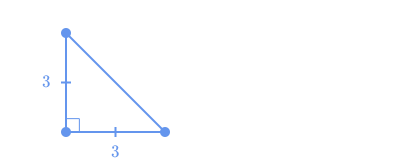
\includegraphics[scale=\shrinkfactor]{figures/29740936508e0ec4c2d3167e2aec0f3372ce78bf.png}



\medskip
\noindent
\textbf{Tags:} {\footnotesize Constructing triangles, CC.7.G.A.2}\\
\textbf{Version:} 2e87ab50.. 2013-10-17
\smallskip\hrule





\section{\href{https://www.khanacademy.org/devadmin/content/items/x651844ecfaac48e9}{x651844ecfaac48e9}}

\noindent
**Draw a right triangle with two $45^\circ$ angles.**

**Given these criteria is the triangle unique?**
[[? interactive-graph 1]]

\paragraph{Ans} 

Yes

\fbox{ No

}

 

\paragraph{Hint 1}Let�s start by drawing. A right triangle has one $\blue{90 ^\circ}$ angle. 

We have an isosceles right triangle. An isosceles right triangle has at least $2$ side lengths equal and $2$ $\blue{45 ^\circ}$ angles.

\paragraph{Hint 2}We know the measure of all $3$ angles but not the length of any side. We can draw many triangles of various sizes all with a pair of $\blue{45 ^\circ}$ angles.

\paragraph{Hint 3}The triangle is not unique.

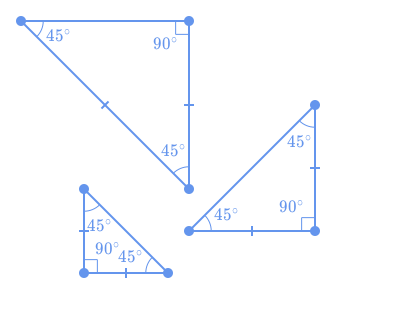
\includegraphics[scale=\shrinkfactor]{figures/91996cb5320f958d2fa0f8249c77e9d88bbb2764.png}



\medskip
\noindent
\textbf{Tags:} {\footnotesize Constructing triangles, CC.7.G.A.2}\\
\textbf{Version:} 85d97ee1.. 2013-10-17
\smallskip\hrule





\section{\href{https://www.khanacademy.org/devadmin/content/items/x6763ceb1ec0ceb41}{x6763ceb1ec0ceb41}}

\noindent
**How many triangles can be drawn where the lengths of all $3$ sides are known?**

\paragraph{Ans} 

None

\fbox{ Only one

}

 More than one



\paragraph{Hint 1}A triangle is a plane figure with $3$ straight sides and $3$ angles. Can we satisfy the definition given the conditions? Let's try to draw a triangle where we known the lengths of all $3$ sides.

\paragraph{Hint 2}For example, let's look at when all side lengths are $\blue1$. We have an equilateral triangle with equal sides and equal angles:


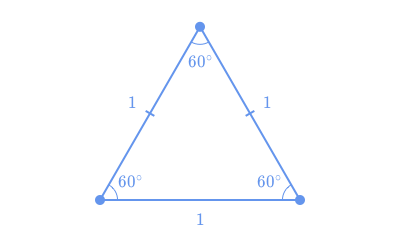
\includegraphics[scale=\shrinkfactor]{figures/b0e7ebe35f997eac2f27bbad47f0033422d118b3.png}

This triangle is unique, meaning no other triangle exists with exact same shape or size.

\paragraph{Hint 3}If the lengths of all $3$ sides are known, only one triangle can be drawn.



\medskip
\noindent
\textbf{Tags:} {\footnotesize Constructing triangles, CC.7.G.A.2}\\
\textbf{Version:} def3450f.. 2013-10-18
\smallskip\hrule





\section{\href{https://www.khanacademy.org/devadmin/content/items/x67ee6010588311f2}{x67ee6010588311f2}}

\noindent
**How many triangles can be drawn with side lengths $4$, $6$ and $10$?**

\paragraph{Ans} 

\fbox{ None

}

 Only one

More than one



\paragraph{Hint 1}A triangle is a plane figure with $3$ straight sides and $3$ angles. Can we satisfy the definition given the conditions? Let's try to draw a triangle given the conditions.

\paragraph{Hint 2}In general, the longest side of a triangle must be shorter than the sum of the two other sides. Because $\blue{4}+\blue{6} =\blue{10}$, the two sides $\blue{4}$ and $\blue{6}$ cannot meet to form a third angle. We cannot create $3$ angles to satisfy the definition of a triangle.


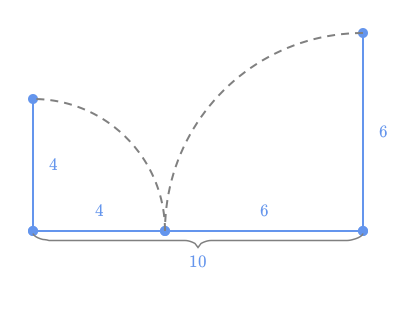
\includegraphics[scale=\shrinkfactor]{figures/acf337830bf93b0d2118eb2712a2d821a3ddd4c1.png}

\paragraph{Hint 3}Given the conditions, no triangles can be drawn.



\medskip
\noindent
\textbf{Tags:} {\footnotesize Constructing triangles, CC.7.G.A.2}\\
\textbf{Version:} 9421cd19.. 2013-10-18
\smallskip\hrule





\section{\href{https://www.khanacademy.org/devadmin/content/items/x67fd10caf4f54df2}{x67fd10caf4f54df2}}

\noindent
**Draw a triangle with side lengths $3a$,  $4a$ and $5a$ where $a>0$.**

**Given these criteria is the triangle unique?**
[[? interactive-graph 1]]

\paragraph{Ans} 

Yes

\fbox{ No

}

 

\paragraph{Hint 1}Let�s start by choosing a value for $\pink{a}$ where $\pink{a}>0$, then we can draw a triangle with side lengths $\purple3\pink{a}$, $\purple4\pink{a}$ and $\purple5\pink{a}$.

\paragraph{Hint 2}If $\pink{a}=1$, then we can draw a triangle with side lengths $\blue3$, $\blue4$ and $\blue5$. This is a right triangle.

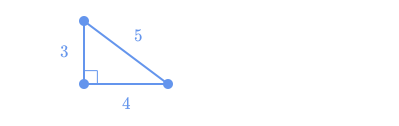
\includegraphics[scale=\shrinkfactor]{figures/b1eff2246ff6077c50f40ea6bfe55bad4b8ced80.png}

\paragraph{Hint 3}If $\pink{a}=2$, then we can draw a right triangle with side lengths $\blue6$, $\blue8$ and $\blue{10}$. 

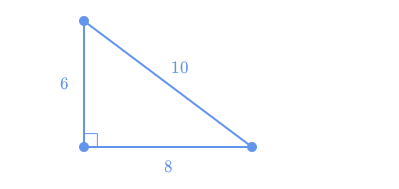
\includegraphics[scale=\shrinkfactor]{figures/ef5a8edbd9d4f5680b124ce81e7f4c78a9707ed4.png}

We can let $\pink{a}$ be any nonzero positive number and draw many triangles of same shape but different sizes.

\paragraph{Hint 4}The triangle is not unique. 


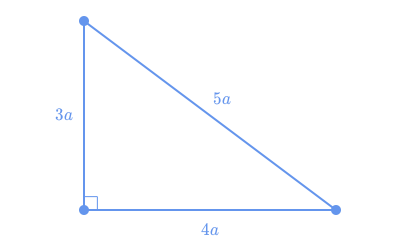
\includegraphics[scale=\shrinkfactor]{figures/946760cec54502326e2f2708bb7c84428118c9ad.png}



\medskip
\noindent
\textbf{Tags:} {\footnotesize Constructing triangles, CC.7.G.A.2}\\
\textbf{Version:} 196bcc1a.. 2013-10-18
\smallskip\hrule





\section{\href{https://www.khanacademy.org/devadmin/content/items/x6d7be6276bcb5815}{x6d7be6276bcb5815}}

\noindent
**Draw a right triangle with a height of $4$ and base of $5$.** 

**Given these criteria is the triangle unique?**
[[? interactive-graph 1]]

\paragraph{Ans} 

\fbox{ Yes

}

 No



\paragraph{Hint 1}Let�s start by drawing. A right triangle has a $\blue{90 ^\circ}$angle. 

The height of length $\blue{4}$ is drawn vertically (up and down) from the $\blue{90 ^\circ}$angle. The base of length $\blue{5}$ is drawn horizontally (left and right) from the $\blue{90 ^\circ}$angle. 

\paragraph{Hint 2}Since we are given the measures of $2$ sides and the angle between them, we can draw only $1$ triangle.

\paragraph{Hint 3}The triangle is unique.


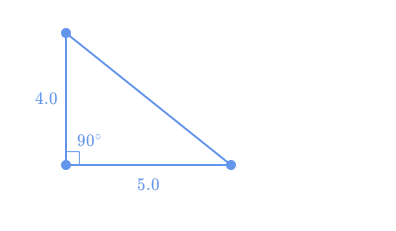
\includegraphics[scale=\shrinkfactor]{figures/21924a4df5c1451289595e8ec2c9ceae30ed7de1.png}



\medskip
\noindent
\textbf{Tags:} {\footnotesize Constructing triangles, CC.7.G.A.2}\\
\textbf{Version:} cf653e34.. 2013-10-17
\smallskip\hrule





\section{\href{https://www.khanacademy.org/devadmin/content/items/x72d893d1e3229dfd}{x72d893d1e3229dfd}}

\noindent
**How many triangles can be drawn side lengths of $3$ and $4$?**

\paragraph{Ans} 

None

Only one

\fbox{ More than one

}

 

\paragraph{Hint 1}Without knowing at least $1$ angle measure, we cannot create a unique triangle with only one shape and size.

\paragraph{Hint 2}We can  draw many triangles with side lengths $\blue3$ and $\blue{4}$.


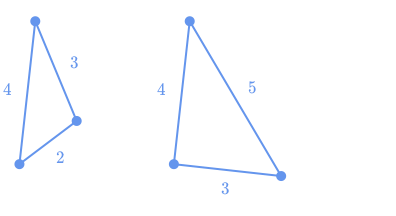
\includegraphics[scale=\shrinkfactor]{figures/2d99bebb2da26f68f4d74679d523ed8d96db3e5c.png}

\paragraph{Hint 3}If we only know $1$ angle and $1$ side length, more than one triangle can be drawn.



\medskip
\noindent
\textbf{Tags:} {\footnotesize Constructing triangles, CC.7.G.A.2}\\
\textbf{Version:} 58c104bc.. 2013-10-18
\smallskip\hrule





\section{\href{https://www.khanacademy.org/devadmin/content/items/x892857b71e427c39}{x892857b71e427c39}}

\noindent
**How many triangles can be drawn with angles $60^\circ$,  $60^\circ$ and $70^\circ$?**

\paragraph{Ans} 

\fbox{ None

}

 Only one

More than one



\paragraph{Hint 1}A triangle is a plane figure with $3$ straight sides and $3$ angles. The $3$ angles always add up to $\pink{180^\circ}$.

\paragraph{Hint 2}Let's add together the angles angles $\blue{60}^\circ$,  $\blue{60}^\circ$ and $\blue{70}^\circ$:

\begin{align*} &= 2\cdot\blue{60^\circ}+\blue{70^\circ}\\
&= 120^\circ+\blue{70^\circ}\\&= 190^\circ\\&>\pink{180^\circ}\end{align*}

The $3$ angles sum up to a value greater than $\pink{180^\circ}$.

\paragraph{Hint 3}Given the conditions, no triangles can be drawn.



\medskip
\noindent
\textbf{Tags:} {\footnotesize Constructing triangles, CC.7.G.A.2}\\
\textbf{Version:} bc3efef4.. 2013-10-18
\smallskip\hrule





\section{\href{https://www.khanacademy.org/devadmin/content/items/xb9aa47b3de982d55}{xb9aa47b3de982d55}}

\noindent
**Draw an isosceles triangle with two $70^\circ$ angles.**

**Given these criteria is the triangle unique?**
[[? interactive-graph 1]]

\paragraph{Ans} 

Yes

\fbox{ No

}

 

\paragraph{Hint 1}Let�s start by drawing an isosceles triangle with $2$ $\blue{70^\circ}$ angles. An isosceles triangle has at least $2$ side lengths equal and $2$ angles equal.

\paragraph{Hint 2}We do not know the side lengths, so we can draw many triangles.

\paragraph{Hint 3}The triangle is not unique.

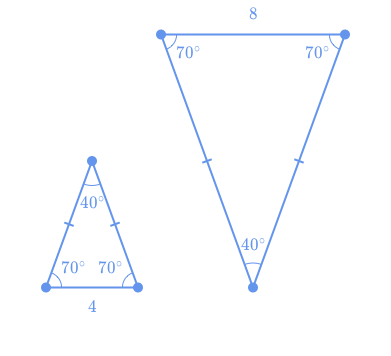
\includegraphics[scale=\shrinkfactor]{figures/afb29f0a848d89c4b6991b76cd2f1a48e594243b.png}



\medskip
\noindent
\textbf{Tags:} {\footnotesize Constructing triangles, CC.7.G.A.2}\\
\textbf{Version:} 5f43d2fc.. 2013-10-17
\smallskip\hrule





\section{\href{https://www.khanacademy.org/devadmin/content/items/xbd061a8700fced6c}{xbd061a8700fced6c}}

\noindent
**How many right triangles can be drawn with angles $40^\circ$ and  $60^\circ$?**

\paragraph{Ans} 

\fbox{ None

}

 Only one

More than one



\paragraph{Hint 1}A triangle is a plane figure with $3$ straight sides and $3$ angles. The $3$ angles always add up to $\pink{180^\circ}$.

A right triangle has a $\blue{90}^\circ$  angle.

\paragraph{Hint 2}Let's add together the angles angles $\blue{40}^\circ$,  $\blue{60}^\circ$ and $\blue{90}^\circ$:

\begin{align*} &=  \blue{40^\circ}+\blue{60^\circ}+\blue{90^\circ}\\
&= 190^\circ\\&>\pink{180^\circ}\end{align*}

The $3$ angles sum up to a value greater than $\pink{180^\circ}$.

\paragraph{Hint 3}Given the conditions, no triangles can be drawn.



\medskip
\noindent
\textbf{Tags:} {\footnotesize Constructing triangles, CC.7.G.A.2}\\
\textbf{Version:} aabc8e4a.. 2013-10-18
\smallskip\hrule





\section{\href{https://www.khanacademy.org/devadmin/content/items/xc001c788d01d9e5f}{xc001c788d01d9e5f}}

\noindent
**Draw a triangle where side length $4$ is not between two angles $58^\circ$ and $90^\circ$.**

**Given these criteria is the triangle unique?**
[[? interactive-graph 1]]

\paragraph{Ans} 

\fbox{ Yes

}

 No



\paragraph{Hint 1}Let�s start by drawing a right angle which is $\blue{90^\circ}$. 

Then, let's draw the side of length $\blue4$ next to the right angle, so our base has a length of $\blue4$.

\paragraph{Hint 2}The side of length $\blue4$ is $\red{\text{not}}$ between $2$ angles $\blue{58^\circ}$ and $\blue{90^\circ}$. 

Since we drew the side of length $\blue4$ next to the right angle, the $\blue{58^\circ}$ angle must be *opposite* the side of length $\blue4$ .

\paragraph{Hint 3}We know the measure of $2$ angles and the length of $1$ side not between the angles, so we can draw only $1$ triangle.

\paragraph{Hint 4}The triangle is unique.


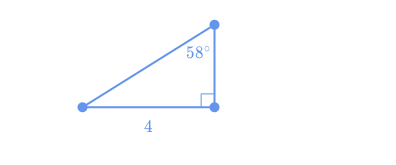
\includegraphics[scale=\shrinkfactor]{figures/0ddd88656709215709e4a46913277db7929349d4.png}



\medskip
\noindent
\textbf{Tags:} {\footnotesize Constructing triangles, CC.7.G.A.2}\\
\textbf{Version:} 9534c031.. 2013-10-17
\smallskip\hrule





\section{\href{https://www.khanacademy.org/devadmin/content/items/xc256611ab7d92e83}{xc256611ab7d92e83}}

\noindent
**Draw a triangle with side length $5$ between two $58^\circ$ angles.** 

**Given these criteria is the triangle unique?**
[[? interactive-graph 1]]

\paragraph{Ans} 

\fbox{ Yes

}

 No



\paragraph{Hint 1}Let�s start by drawing the length of $1$ side, which we know is $\blue5$.  

\paragraph{Hint 2}From the side $\blue5$, let�s draw $2$ $\blue{58^\circ}$ angles. Since we have $2$ equal angles, we have an isosceles triangle. An isosceles triangle has at least $2$ sides equal in length. 

Since we have $2$ $\blue{58^\circ}$ angles, the third angle must be $\green{64^\circ}$. The sum of $3$ angles in a triangle will always be $\pink{180^\circ}$.

\paragraph{Hint 3}We know the measure of $2$ angles and the length of the side between the angles, so we can draw only $1$ triangle.

\paragraph{Hint 4}The triangle is unique.


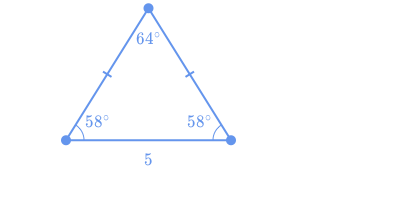
\includegraphics[scale=\shrinkfactor]{figures/4af5c292b250f14e2725fbff73825f6e41348a27.png}



\medskip
\noindent
\textbf{Tags:} {\footnotesize Constructing triangles, CC.7.G.A.2}\\
\textbf{Version:} 5ba2ed08.. 2013-10-17
\smallskip\hrule





\section{\href{https://www.khanacademy.org/devadmin/content/items/xc40b1278855716df}{xc40b1278855716df}}

\noindent
**Draw a triangle with side lengths $3$, $4$ and $5$.** 

**Given these criteria is the triangle unique?**
[[? interactive-graph 1]]

\paragraph{Ans} 

\fbox{ Yes

}

 No



\paragraph{Hint 1}Let�s start by drawing. We know the lengths of all $3$ sides. How many triangles can we draw?

\paragraph{Hint 2}The triangle with side lengths $\blue3$, $\blue4$ and $\blue5$ is a right triangle. Since we are given the measures of $3$ sides, we can draw only $1$ triangle. 

\paragraph{Hint 3}The triangle is unique.


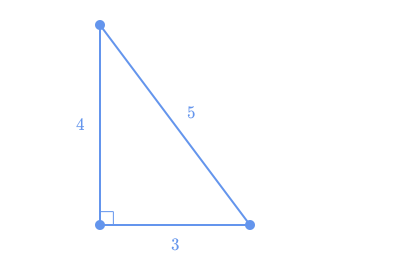
\includegraphics[scale=\shrinkfactor]{figures/758d66a2a3006feaf0b6d196067ab8a9e5a4c587.png}



\medskip
\noindent
\textbf{Tags:} {\footnotesize Constructing triangles, CC.7.G.A.2}\\
\textbf{Version:} b5262e6e.. 2013-10-17
\smallskip\hrule





\section{\href{https://www.khanacademy.org/devadmin/content/items/xcfae18d2af4efa34}{xcfae18d2af4efa34}}

\noindent
**Draw a scalene triangle with angles $45^\circ$,  $60^\circ$ and $75^\circ$.**

**Given these criteria is the triangle unique?**
[[? interactive-graph 1]]

\paragraph{Ans} 

Yes

\fbox{ No

}

 

\paragraph{Hint 1}Let�s start by drawing. While keeping $1$ angle, we can change the side lengths to create $1$ of the other $2$ angles.

For example, while keeping a $\blue{60^\circ}$ angle, we can change the side lengths to create the $\blue{45^\circ}$ angle. The final angle will be $\blue{75^\circ}$.

\paragraph{Hint 2}We know the measure of $3$ angles but not the length of any side. We can draw many triangles of the same shape but different sizes.

\paragraph{Hint 3}The triangle is not unique.


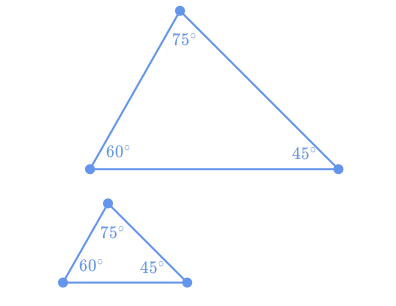
\includegraphics[scale=\shrinkfactor]{figures/2a7061cde7a64397a1147db0b6c38402785f7ab0.png}



\medskip
\noindent
\textbf{Tags:} {\footnotesize Constructing triangles, CC.7.G.A.2}\\
\textbf{Version:} 5ef1e69a.. 2013-10-18
\smallskip\hrule





\section{\href{https://www.khanacademy.org/devadmin/content/items/xdba9a2b900c8bbcd}{xdba9a2b900c8bbcd}}

\noindent
**How many triangles can be drawn with side lengths $1$, $2$ and $3$?**

\paragraph{Ans} 

\fbox{ None

}

 Only one

More than one



\paragraph{Hint 1}A triangle is a plane figure with $3$ straight sides and $3$ angles. Can we satisfy the definition given the conditions? Let's try to draw a triangle given the conditions.

\paragraph{Hint 2}In general, the longest side of a triangle must be shorter than the sum of the two other sides. Because $\blue{1}+\blue{2} =\blue{3}$, the two sides $\blue{1}$ and $\blue{2}$ cannot meet to form a third angle. We cannot create $3$ angles to satisfy the definition of a triangle.


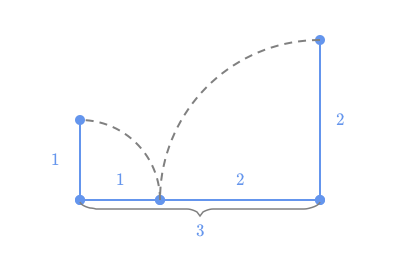
\includegraphics[scale=\shrinkfactor]{figures/8138125d70973033dceda459b359bd456038254f.png}

\paragraph{Hint 3}Given the conditions, no triangles can be drawn.



\medskip
\noindent
\textbf{Tags:} {\footnotesize Constructing triangles, CC.7.G.A.2}\\
\textbf{Version:} 2feadc91.. 2013-10-18
\smallskip\hrule





\section{\href{https://www.khanacademy.org/devadmin/content/items/xe06107bc78ca0b3c}{xe06107bc78ca0b3c}}

\noindent
**How many triangles can be drawn with angles $30^\circ$,  $50^\circ$ and $100^\circ$?**

\paragraph{Ans} 

None

Only one

\fbox{ More than one

}

 

\paragraph{Hint 1}We know the measure of $3$ angles but not the length of any side. We can draw many triangles with the same shape but different size.

\paragraph{Hint 2}
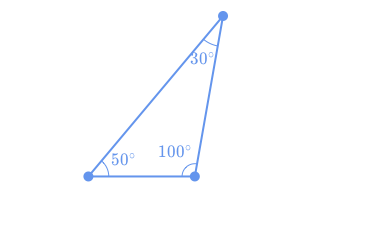
\includegraphics[scale=\shrinkfactor]{figures/cfa8c2afddab68081b192038f3130d47880b443e.png}

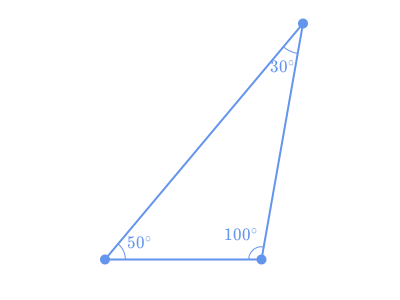
\includegraphics[scale=\shrinkfactor]{figures/b1683148f0f59becb3f7ee5221cd130e632609d7.png}

\paragraph{Hint 3}If the measures of all $3$ angles are known, more than one triangle can be drawn.



\medskip
\noindent
\textbf{Tags:} {\footnotesize Constructing triangles, CC.7.G.A.2}\\
\textbf{Version:} a599ba59.. 2013-10-18
\smallskip\hrule





\section{\href{https://www.khanacademy.org/devadmin/content/items/xe937d430ba8d75d8}{xe937d430ba8d75d8}}

\noindent
**How many triangles can be drawn with one $45^\circ$ and a side length of $5$?**

\paragraph{Ans} 

None

Only one

\fbox{ More than one

}

 

\paragraph{Hint 1}A triangle is a plane figure with $3$ straight sides and $3$ angles. 

The $3$ angles always add up to $\pink{180^\circ}$. We only know $1$ angle is $\blue{45^\circ}$. We can't find the measures of the other $2$ angles.

\paragraph{Hint 2}We know the length of only $1$ side is $\blue5$. Depending if we place the side of length $\blue5$ next to or across from the $\blue{45^\circ}$ angle, we can  draw many triangles with different shapes and different sizes.


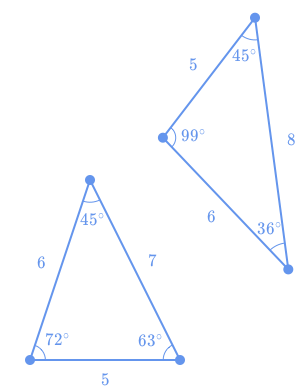
\includegraphics[scale=\shrinkfactor]{figures/8fd2ab6db3cbbe9cbdf43af4cf872835fa89ecf2.png}

\paragraph{Hint 3}If we only know $1$ angle and $1$ side length, more than one triangle can be drawn.



\medskip
\noindent
\textbf{Tags:} {\footnotesize Constructing triangles, CC.7.G.A.2}\\
\textbf{Version:} 82a35698.. 2013-10-18
\smallskip\hrule





\section{\href{https://www.khanacademy.org/devadmin/content/items/xf51994a651ca1d7f}{xf51994a651ca1d7f}}

\noindent
**Draw a triangle with angles $30^\circ$,  $50^\circ$ and $100^\circ$.**

**Given these criteria is the triangle unique?**
[[? interactive-graph 1]]

\paragraph{Ans} 

Yes

\fbox{ No

}

 

\paragraph{Hint 1}Let�s start by drawing. While keeping $1$ angle, we can change the side lengths to create $1$ of the other $2$ angles.

While keeping a $\blue{100^\circ}$ angle, we can change the side lengths to create the $\blue{50^\circ}$ angle. The final angle will be $\blue{30^\circ}$.

\paragraph{Hint 2}We know the measure of $3$ angles but not the length of any side. We can draw many triangles of same shape but different sizes.

\paragraph{Hint 3}The triangle is not unique.

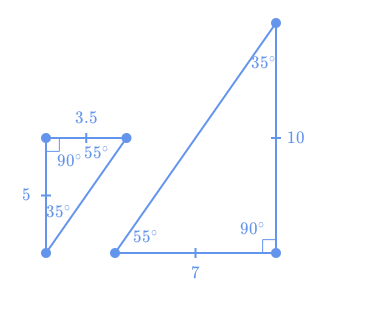
\includegraphics[scale=\shrinkfactor]{figures/13ed90e8845185b7c961687bdf49c22135f67ec5.png}



\medskip
\noindent
\textbf{Tags:} {\footnotesize Constructing triangles, CC.7.G.A.2}\\
\textbf{Version:} ac2e7f53.. 2013-10-18
\smallskip\hrule





\section{\href{https://www.khanacademy.org/devadmin/content/items/xf9872931929ac56c}{xf9872931929ac56c}}

\noindent
**Draw a triangle with side lengths $5$, $12$ and $13$.** 

**Given these criteria is the triangle unique?**
[[? interactive-graph 1]]

\paragraph{Ans} 

\fbox{ Yes

}

 No



\paragraph{Hint 1}Let�s start by drawing. We know the lengths of all $3$ sides. How many triangles can we draw?

\paragraph{Hint 2}Since we are given the measures of $3$ sides, we can draw only $1$ triangle. The triangle with side lengths $\blue5$, $\blue{12}$ and $\blue{13}$ is a right triangle.

\paragraph{Hint 3}The triangle is unique.


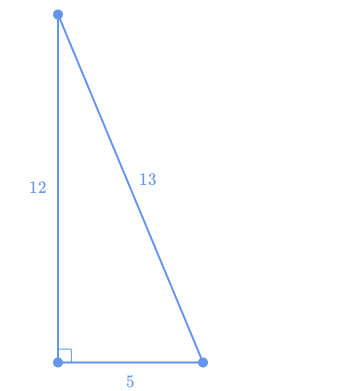
\includegraphics[scale=\shrinkfactor]{figures/227ab289b1de518857460dab83b70e050be9fa46.png}



\medskip
\noindent
\textbf{Tags:} {\footnotesize Constructing triangles, CC.7.G.A.2}\\
\textbf{Version:} 18374b72.. 2013-10-17
\smallskip\hrule



%%  Create a directory called 'figures' in latex dir and run the following command 
%  wget -N \
%    https://ka-perseus-graphie.s3.amazonaws.com/8664b06c420b8bf33711310103a6963e0f2cc7f1.png \
%    https://ka-perseus-graphie.s3.amazonaws.com/9e3335e4646b2e59f3ceb8860cd9099de97f22b0.png \
%    https://ka-perseus-graphie.s3.amazonaws.com/6d298ed14c507f692b6d88792d963d7008b9847a.png \
%    https://ka-perseus-graphie.s3.amazonaws.com/463955e595c31361c49d853aea12289b0f5f7779.png \
%    https://ka-perseus-graphie.s3.amazonaws.com/28bab6f73b266fa0cb6392a48f06caca532f0cd2.png \
%    https://ka-perseus-graphie.s3.amazonaws.com/42e1efd00be59b64d19c796b09c66213066bd2fa.png \
%    https://ka-perseus-graphie.s3.amazonaws.com/fe9bb66c73daee381242a48159a578e8b78ac0fb.png \
%    https://ka-perseus-graphie.s3.amazonaws.com/50ab52075216ec1ebe030aa80de8615558c71846.png \
%    https://ka-perseus-graphie.s3.amazonaws.com/48773248b446b970cdf6c2fa7664c3fa8890378a.png \
%    https://ka-perseus-graphie.s3.amazonaws.com/a5961a517a4e6e5e6def530e3948dc049dbfad9a.png \
%    https://ka-perseus-graphie.s3.amazonaws.com/0fc8a765d9e1e79a7c3e4874b8f9448d3b5c1d18.png \
%    https://ka-perseus-graphie.s3.amazonaws.com/d8b2dd5b2d43266692ba3d2c35cf5638f2f3c05c.png \
%    https://ka-perseus-graphie.s3.amazonaws.com/9bbd0fa30a5ae16d50c816c4a8c4cfc44a68146c.png \
%    https://ka-perseus-graphie.s3.amazonaws.com/3e0462daa95058cdd7264a43f9c163723c418fd6.png \
%    https://ka-perseus-graphie.s3.amazonaws.com/29740936508e0ec4c2d3167e2aec0f3372ce78bf.png \
%    https://ka-perseus-graphie.s3.amazonaws.com/91996cb5320f958d2fa0f8249c77e9d88bbb2764.png \
%    https://ka-perseus-graphie.s3.amazonaws.com/b0e7ebe35f997eac2f27bbad47f0033422d118b3.png \
%    https://ka-perseus-graphie.s3.amazonaws.com/acf337830bf93b0d2118eb2712a2d821a3ddd4c1.png \
%    https://ka-perseus-graphie.s3.amazonaws.com/b1eff2246ff6077c50f40ea6bfe55bad4b8ced80.png \
%    https://ka-perseus-graphie.s3.amazonaws.com/ef5a8edbd9d4f5680b124ce81e7f4c78a9707ed4.png \
%    https://ka-perseus-graphie.s3.amazonaws.com/946760cec54502326e2f2708bb7c84428118c9ad.png \
%    https://ka-perseus-graphie.s3.amazonaws.com/21924a4df5c1451289595e8ec2c9ceae30ed7de1.png \
%    https://ka-perseus-graphie.s3.amazonaws.com/2d99bebb2da26f68f4d74679d523ed8d96db3e5c.png \
%    https://ka-perseus-graphie.s3.amazonaws.com/afb29f0a848d89c4b6991b76cd2f1a48e594243b.png \
%    https://ka-perseus-graphie.s3.amazonaws.com/0ddd88656709215709e4a46913277db7929349d4.png \
%    https://ka-perseus-graphie.s3.amazonaws.com/4af5c292b250f14e2725fbff73825f6e41348a27.png \
%    https://ka-perseus-graphie.s3.amazonaws.com/758d66a2a3006feaf0b6d196067ab8a9e5a4c587.png \
%    https://ka-perseus-graphie.s3.amazonaws.com/2a7061cde7a64397a1147db0b6c38402785f7ab0.png \
%    https://ka-perseus-graphie.s3.amazonaws.com/8138125d70973033dceda459b359bd456038254f.png \
%    https://ka-perseus-graphie.s3.amazonaws.com/cfa8c2afddab68081b192038f3130d47880b443e.png \
%    https://ka-perseus-graphie.s3.amazonaws.com/b1683148f0f59becb3f7ee5221cd130e632609d7.png \
%    https://ka-perseus-graphie.s3.amazonaws.com/8fd2ab6db3cbbe9cbdf43af4cf872835fa89ecf2.png \
%    https://ka-perseus-graphie.s3.amazonaws.com/13ed90e8845185b7c961687bdf49c22135f67ec5.png \
%    https://ka-perseus-graphie.s3.amazonaws.com/227ab289b1de518857460dab83b70e050be9fa46.png \


\end{document}

